\chapter{Project Introduction}
\section{Project Overview}
This chapter provides an overview to my project. Firstly defining usability in the context of \gls{hci} and the \gls{ta} methodology. This is followed by the introduction of my research aims and objectives of this project, as well as the research questions that I hope to answer from my conducted research. Additionally, I have provided a description of each chapter present in this work.

\section{Usability Background}
The usability of a product or service is of the utmost importance, if a user cannot easily use the service then its functionality becomes all the more meaningless. There are however several methods used to assess the ease of use of a product, including usability testing and heuristic evaluation. Usability testing is an ever changing field due to the diverse nature of products and services we all use, with various methodologies on how to conduct usability studies, such as the ``Think-Aloud" (TA) concept. The Think-Aloud concept can then be further divided into different variants. The two most common variants are \gls{cta} and \gls{rta}. The simple difference between these two variants is that CTA methods ask the test participant to verbalise there thoughts whilst they are in the process of completing tasks. In contrast, RTA methods ask the user to complete the task and then describe the thought process after the testing. CTA and RTA can also be combined into a Hybrid methodology, however this is used to a lesser extent than the more classical methods \citep{alhadreti2016thinking}. Additionally the way in which participants are selected can also greatly effect the results of the study. For instance a study could revolve around that of the users age, and how different aged users interact with a program, website or service, although there are many other aspects that could be analysed or have influence in a usability study \citep{rubin2008handbook}. However, for this project the influence that a users previous experience will be analysed during a concurrent Think-aloud study. 


\section{Research Aims, Objectives and Questions}
\subsection{Project Aim}
The main aim of my project will be to analyse the relationship that a users experience has on the concurrent think-aloud usability methodology. Certain studies point out the issues that concurrent think-aloud can have on the validity of data, as it can distract users from trying to complete tasks, especially if they are a novice user of a service. Therefore by testing the previous knowledge and experience that users have, I will study whether this has a great effect on the data sets collected. My null hypothesis for this project will be that there is no difference between Novice and Experienced Users regarding Issues encountered in type or frequency.

\subsection{Project Objective}
In order to achieve this aim, I will need to achieve the following objectives (OBJX). 

\begin{figure}[H]
    \centering
    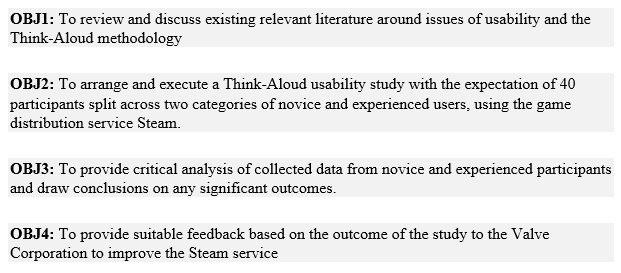
\includegraphics{Screenshots/projectObjectives.png}
\end{figure} 
   
   
   
    
\subsection{Research Questions}
During my project I will attempt too answer the following research questions (RQX). These research questions will be discussed within Chapter 6, Research Discussion. 

\begin{figure}[H]
    \centering
    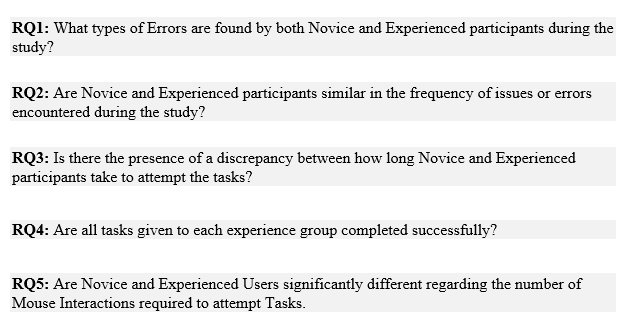
\includegraphics{Screenshots/rqxUpdated.png}
\end{figure}



\section{Structure of this work}
This work will be split into multiple chapters. This chapter, chapter 1 is an introduction to this work, introducing themes of UX research, usability and my projects overall aims, objectives and research questions. Chapter 2, Literature Review, provides a further look into the existing materials for both \gls{ta} methodology, but also for work relating to previous user knowledge and the influence can have upon TA research. Chapter 3, Research Methodology, is an overview on my my UX research was conducted, including what materials, participant criteria and data that I collected as part of this work. Chapter 4, Participant Demographics, presents all of my data collected on my Novice and Experienced participants, including factors such as generic demographics including age, gender and education, secondly questions relating to participant previous experience with gaming such as how many hours spent playing games by each type of participant. Chapter 5, Research Findings, is the presentation of my data collected from my study, with the following data metrics, issue and error detection, Task Duration, Task Completion and Task Mouse Interactions. Chapter 6 Results Discussion, takes this all data sets collected and evaluates the results in context of the research questions presented in Chapter 1.3. Lastly, Chapter 7 Conclusion, summarises the project and presents its limitations and finally suggests some new aspects for further study and expansion on this work.


